% write your main thesis in logical individual chapters
% for better organization use a separate folder for images
\graphicspath{{img/}}








%==============================
\chapter{Pregled metod medplaformnega razvoja}
\label{chap:overview}

Predno postavimo omejitve razvoja naše aplikacije, si poglejmo različne metode medplatformnega razvoja in v katerih primerih jih je pametno uporabiti. Kot je pričakovati, jih je kar nekaj. Razdelili jih bomo v skupine celovitih, delnih in deljenih metod.

%-----
\section{Celovit}

Celovita metoda za razvoj uporablja ogrodje, s pomočjo katerega aplikacijo pripravimo za različne platforme. Velika večina tako napisane izvorne kode je uporabljena na vseh destinacijskih platformah, za kar poskrbi ogrodje. Rezultat te metode je domorodna aplikacija (\eng{native application}), ki jo je možno objaviti v trgovinah posameznih platform in pri tem ne kršijo (ponavadi) strogih pravil.

\subsection{Qt}

Qt\cite{qt} je ogrodje za grafično programiranje za več platform s pomočjo jezika C++ in QML\footnote{Qt Meta Language ali Qt Modeling Language}. Omogoča nam sočasni razvoj za platforme OSX, Linux, Windows, Android in iOS. Podpira tudi uporabo HTML5 namesto QML, kar pomeni, da spletni razvijalci lahko uporabijo že obstoječe znanje in učenje novega jezika ni potrebno.

Qt projekt je povsem odprtokoden in dovoljuje uporabo v skladu z licencama GPL v3\cite{gpl} in LGPL v2.1\cite{lgpl}, a če želite orodje uporabiti za razvoj mobilne aplikacije, boste morali za to odšteti 149\$ mesečno.

Projekt so vrsto let uspešno razvijali v podjetju Nokia, kjer so ga uporabili kot glavno orodje za razvoj aplikacij na platformi Symbian. Ko je pred časom Microsoft kupil podjetje Nokia, je projekt prevzela novonastala organizacija Qt Project, ki projekt vodi še danes.

Qt je še posebej privlačen zaradi podpore namiznih platform kot so Windows, Mac OSX in Linux. Odlikuje ga tudi zagreta skupnost razvijalcev.

Ogrodje Qt je primeren za izdelavo aplikacij, ki vključujejo kompleksne algoritme, za katere bi porabili preveč časa pri prepisovanju na različne platforme. Lep primer tega sta aplikaciji Mathematica\cite{mathematica} in multimedijski predvajalnik VLC\cite{vlc}.

Glavne slabosti Qt so neskladnost z izgledom ostalih aplikacij na mobilnih platformah, plačljiva licenca za razvoj mobilnih aplikacij ter končna velikost samih programov. Manjka tudi napovedana podpora za platformo Windows Phone.

\subsection{Xamarin}

Xamarin\cite{xamarin} je ogrodje za sočasen razvoj aplikacij za platforme iOS, Android, Mac in Windows v jeziku C\#. Izjaha iz projekta Mono\cite{mono}, ki omogoča uporabo ogrodja .NET na različnih platformah. Ogrodje omogoča razvoj aplikacij, katerih izgled je skladen z ostalimi domorodnimi aplikacijami.

Ogrodje odlikuje integrirano razvojno okolje (IDE), ki razvoj aplikacij znatno olajša. Omogoča testiranje tako v emulatorju/simulatorju, kot na samih napravah.

Xamarin je primeren za izdelavo aplikacij za več različnih platform, kjer je ključnega pomena končna grafična skladnost z ostalimi domorodnimi aplikacijami. Kot primer si lahko ogledamo aplikacijo za poslušanje glasbe Rdio\cite{rdio}, ki je na voljo za iOS, Android in Windows Phone.

Glavna slabost ogrodja Xamarin je cena, saj se paketi začnejo šele pri 299\$/mesec za vsakega razvijalca in vsako platformo posebej. Za majhno ekipo je lahko taka začetna cena enostavno previsoka. Vprašljiva je tudi hitrost dodajanja funckionalnosti posameznih platform, ko se te nadgradijo, določen riziko predstavlja tudi muhavost posameznih platform pri omejitvah uporabe tega ogrodja, sploh če nadgradnja povzroči nedelovanje takih aplikacij.

\subsection{Adobe Air}

Adobe Air\cite{adobeair} je brezplačno ogrodje, ki omogoča zagon iste aplikacije na platformah iOS, Android, Mac, Windows in Linux, zagon aplikacije pa je možen tudi iz spletnega brskalnika. Čeprav za razvoj namiznih aplikacij omogoča uporabo HTML in Javascript, je za razvoj mobilnih aplikacij omejen na uporabo jezika ActionScript. V času pisanja diplomske naloge ogrodje ne omogoča zagon na platformi Windows Phone, vendar so razvijalci podporo že napovedali.

Izbor orodja je še posebej uporaben za aplikacije v katerih uporabniški vmesnik ni potrebno prilagajati posamezni platformi. Ravno zaradi tega je orodje priljubljeno med razvijalci iger, ko je naprimer Angry Birds\cite{angrybirds}.

Kot glavno slabost ogrodja Adobe Air bi navedel upadanje zanimanja za orodje Flash. Špekuliramo lahko tudi o planih podjetja Adobe, saj so pred kratkim kupili podjetje Nitobi, ki je avtor ogrodja PhoneGap (katerega si ga bomo ogledali v nadaljevanju). Uporaba tudi ni primerna za razvoj klasičnih mobilinih aplikacij, saj je prilagajanje domorodnim aplikacijam precej zahtevno, še posebej kadar na platformi pride do posodobitve izgleda.

%-----
\section{Hibriden}

Hibridna metoda za razvoj aplikacij uporablja spletne tehnologije v sožitju z kodo za posamezno platformo (t.i. premostitvena tehnika), ki omogoča dostop do glavnih funkcij naprav (kot so kamera, pospeškomer in podobno). Tako kot pri celovitih metodah, je tudi tu rezultat domorodna aplikacija, ki jo je možno objaviti v trgovinah posameznih platform.

\subsection{Apache Cordova / PhoneGap}

Ogrodje Apache Cordova\cite{cordova} je odprtokodni projekt, ki omogoča objavo spletnih aplikacij kot domorodne. V času pisanja diplomske naloge ogrodje podpira iOS, Android, Windows Phone, Blackberry, Palm WebOS, Bada in Symbian. Na vseh omenjenih platformah nam ogrodje Apache Cordova omogoča dostop do funkcij naprave, ko so naprimer kamera in pospeškomer. Isto aplikacijo je možno zagnati tudi v spletnem brskalniku, a je za to potrebno nekaj dodatnega dela.

Projekt PhoneGap\cite{phonegap} je dejansko samo ena od distribucij projekta Apache Cordova, ki poleg vseh obstoječih funkcionalnosti ponuja tudi razne storitve na katerih delajo v podjetju Adobe.

Za razvoj aplikacij razvijalci lahko uporabljajo spletne tehnologije HTML, CSS in JavaScript. S pomočjo ogrodij jQuery Mobile in Sencha Touch je možno izdelati aplikacije, katerih izgled je zelo lep približek ostalim aplikacijam na izbrani platformi. Če naletimo na funkcijo naprave, do katere nimamo dostopa, ali ugotovimo da je JavaScript za določene naloge premalo učinkovit, lahko preprosto spišemo lasten vtičnik, ki služi kot most med kodo napisano v jeziku JavaScript in domorodno kodo.

Glavna prednost ogrodja Apache Cordova in predvsem distribucije PhoneGap je izredno nezahtevnost ogrodja. Priporoča se predvsem za izdelavo prototipnih aplikacij, saj nam omogoča hiter razvoj in iteracijo.

Glavna slabost tega pristopa tiči v performanci in odzivnosti aplikacije, saj ta za prikazovanje izkorišča vgrajeno spletno okno. Trenutno je težko izdelati aplikacije, ki so grafično zahtevnejše, kar pomeni še toliko bolj pereč problem na napravah s slabšimi karakteristikami. Da se aplikacija po izgledu nebi ločila od domorodnih aplikacij je potrebno vložiti kar nekaj dela, na koncu pa bo izurjen uporabnik najbrž vseeno opazil, da je aplikacija malce drugačna. Problem predstavlja tudi zamik podpore novim stilom grafičnih elementov, tako kot se je to zgodilo pri prehodu iz iOS6 na iOS7.

\subsection{Appcelerator Titanium}

Ogrodje Titanium\cite{titanium} nam omogoča izdelavo aplikacij za več platform hkrati s pomočjo JavaScript okolja, ki služi kot abstrakcijska plast med našo aplikacijo in domorodno kodo. Aplikacijo gradimo s pomočjo jezika JavaScript, ki se med uporabo aplikacije izvaja s pomočjo pogona V8\cite{v8} (Android), JavaScriptCore (iOS)\cite{javascriptcore} ali vgrajenega JavaScript okolja (če aplikacijo poganjamo v brskalniku). Za pravilen vizualen izgled skrbijo namestniški elementi, ki uporabljajo domorodne grafične elemente, kar pomeni da vizualno aplikacije ne ločimo od ostalih domorodnih aplikacij. V času pisanja diplomske naloge ogrodje podpira iOS, Android, Blackberry, Tizen in spletne aplikacije.

Glavna prednost ogrodja Titanium ni t.i. način piši enkrat, uporabljaj povosd; njegova prednost je da lahko celotno aplikacijo izdelamo v enem jeziku - JavaScript-u. Le redko se bomo srečali z domorodno kodo, saj ogrodje nudi široko paleto knjižnic.

Prav tako kot PhoneGap, je Titanium še posebej uporaben pri razvoju prototipov aplikacij, kjer je cilj hiter razvoj in predstavitev aplikacije čim večjemu krogu uporabnikov.

Glavna slabost ogrodja je počasno dodajanje novih platform zaradi obsežnosti dela, ki ga tak podvig zahteva. Določene knjižnice za delo z domorodnimi elementi tudi niso najbolj performančne, manjka pa tudi napovedana podpora platformi Windows Phone.

%-----
\section{Deljen}

Deljena metoda za razvoj aplikacij omogoča uporabo dela aplikacijske kode na vseh platformah za katere razvijamo. To lahko naredimo s pomočjo vgradnega skriptnega jezika (Lua), s pomočjo prevajanja iz izbranega programskega jezika v domorodnega (Haxe, XMLVM, emscripten) ali pa z uporabo programskih jezikov C++ ali JavaScript in programskimi ovojev, s katerimi pripravimo knjižnico za vgradnjo v druge platforme.

\subsection{Lua}

Lua\cite{lua} je preprost vgradni skriptni jezik, ki ga odlikuje hitrost izvajanja in procesorska nezahtevnost. Vgradimo ga lahko v platforme Android, iOS, Symbian in Windows Phone, z nekaj potrpljenja pa lahko isto kodo zaženemo tudi v spletni aplikaciji.

Ker gre za skriptni jezik, se znajdemo v zanimiv situaciji kjer združujemo prevajane jezike z interpretiranimi jeziki. Velika prednost tega je hitro odzivanje na napake pri razvoju, saj razvijalcu ni potrebno čakati na prevod kode. Odpira tudi možnost posodobitve vgrajene knjižnice brez posodobitve celotne aplikacije.

Čeprav je jezik Lua preprost za uporabo, se izkaže da za kompleksnejše knjižnice ni primeren. Manjka Unicode podpora, boljša podpora rokovanju z napakami, boljša podpora starejšim verzijam in vgrajen razhroščevalnik (\eng{debugger}).

\subsection{Haxe}

Haxe\cite{haxe} zase pravi, da je večplatformski programski jezik. Razvijalec lahko svojo aplikacijo napiše v jeziku Haxe, nato pa jo s pomočjo prevajalnika prevede v izvorno kodo jezikov PHP, ActionScript, Neko, JavaScript, C++, C\# ali Javo. Nudi tudi dodatne vmesnike za dostop do specifičnih metod ciljnega jezika.

Jezik se je prijel predvsem za razvoj iger, kjer naj bi dolgoročno zamenjal jezik ActionScript, ki ga uporablja orodje Flash.

Glavna slabost uporaba rešitve Haxe je majhna razvijalska skupnost. V primerjavi z ostalimi rešitvami, je ta kar v manjšini. V zadnjem času sicer pridobiva nekaj zagona, a je trenutno vse premalo knjižnic, ki bi bile razvite za to platformo.

\subsection{XMLVM}

XMLVM\cite{xmlvm} spada v isti razred kot Haxe - tako imenovanih prevajalcev iz enega jezika v drugega (ang. cross-compilers), a se XMLVM tega loti na drugačen način. Medtem ko Haxe prevaja na nivoju izvorne kode, XMLVM to počne na nivoju zlogovne kode (ang. byte code). Izvorna koda je lahko napisana za navidezne stroje (ang. virtual machine) JVM, .NET CLI ali Ruby YARV, medtem ko je rezultat delujoč program za JVM, .NET CLI, Javascript, Pyhton, Objective-C in C++.

Projekt izgleda zelo ambiciozen, a vse kaže da je šlo le za akademsko raziskavo, saj je v času pisanja diplome minilo že več ko leto dni odkar se je izvorna koda posodobila. Kljub temu se mi je projekt zdel zanimiv in ga je bilo vredno izpostaviti.

\subsection{C++ in emscripten}

V kolikor nobena od naštetih možnosti ne zadošča našim potrebam, želeli pa bi vseeno imeti deljeno knjižnico, obstaja še ena možnost: uporaba jezika C++\cite{cpp} in projekta emscripten\cite{emscripten}.

C++ je eden izmed najbolj razširjenih programksih jezikov. V času pisanja diplomske naloge zaseda četrto mesto na lestvici najbolj popularnih jezikov \ref{fig:tiobe-index}, pred njim so samo C, Java in Objecitve-C. Uporablja se ga v raznolikih projektih, od prevajalnikov, strežnikov, do video igric.

\begin{figure}
 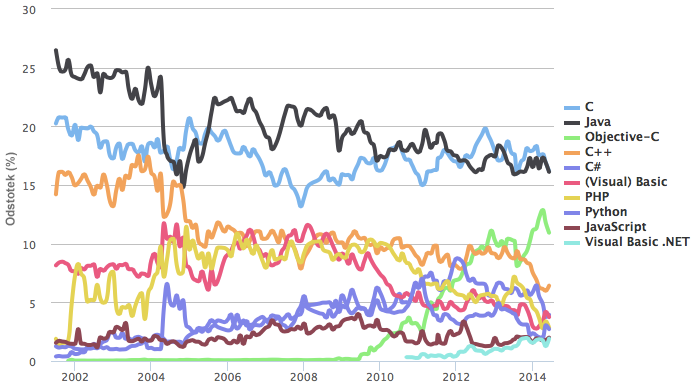
\includegraphics[width=\linewidth]{tiobe-index}
 \caption{Tiobe programming comunity index \cite{tiobe}.}
 \label{fig:tiobe-index}
\end{figure}

Emscripten je projekt Mozilinih laboratorijev, ki omogoča prevajanje iz LLVM\footnote{Low Level Virtual Machine} zlogovne kode v skriptni jezik JavaScript. LLVM si lahko predstavljamo kot vmesni sloj med izvorno (C, C++, Objective-C, Java, C\#) in strojno kodo, ki skrbi poskrbi za visoko optimizacijo vmesne kode, to pa lahko potem prevedemo v ustrezen nabor ukazov za posamezne procesorje (ARM, x86 itd.). Emscripten tako predstavlja zadnjo fazo prevajalnika, le da vmesne kode iz LLVM ne prevede v ukaze specifičnega procesorja, ampak nazaj v jezik JavaScript. To pomeni, da lahko prevedemo skoraj vsak program (z določenimi omejitvami) v JavaScript in ga zaženemo v brskalniku. Celo grafično zahtevne aplikacije\footnote{Skupina Mozilinih inžinirjev je grafično ogrodje Unreal v štirih dneh posodobilo do te mere, da je lahko s pomočjo orodja emscripten grafično zahtevna aplikacija brezhibno delovala v brskalniku\cite{epic-citadel}.} niso problematične, saj emscripten za prevod v JavaScript uporablja asm.js\cite{asmjs}, kar je podmnožica jezika JavaScript, ki jo JavaScript pogoni znajo izredno dobro optimizirati\footnote{S pomočjo asm.js so v podjetju Mozilla uspeli doseči le enkrat počasnejše izvajanje od domorodne kode, kar je izjemen dosežek.\cite{mozilla-asmjs}}.

\subsection{JavaScript}
\label{chap:javascript}

Namesto prevajanja v jezik JavaScript s pomočjo ogrodja Emscripten, bi lahko celotno knjižnico napisali kar v jeziku JavaScript. V zadnjih nekaj letih je jezik JavaScript doživel izredno hitro rast, tako v popularnosti, kot v zmogljivosti in funkcionalnostih, kar je tudi razvidno iz slike \ref{fig:github-jeziki}.

\begin{figure}
 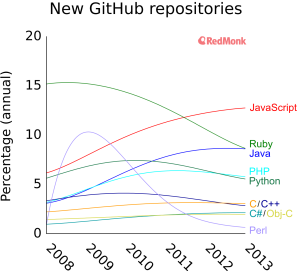
\includegraphics[width=\linewidth]{github-jeziki}
 \caption{Jeziki novih projektov na spletni strani github.com.}
 \label{fig:github-jeziki}
\end{figure}

Pri vključitvi v svojo aplikacijo moramo biti malce bolj iznajdljivi. iOS je z verzijo 7 dodal knjižnico JavaScriptCore, ki omogoča mešanje domorodne in JavaScript kode.

Android je malce bolj problematičen, saj SDK v času pisanja diplomske naloge ne nudi direktne implementacije. Zaradi tega smo primorani vključiti JavaScript pogon, kot je Rhino, V8 in podobni. V kolikor je pogon napisan v jeziku Java, je integracija preprosta, če pa izberemo pogon v drugem jeziku, mora za Android obstajati paket za uvoz.

Windows Phone prav tako kot Android ne nudi JavaScript implementacije, ki bi jo lahko uporabljali skupaj z domorodno kodo. Uporabimo lahko pogon V8 in knjižnico JavaScriptNet\cite{javascriptdotnet}.

Ker je knjižnica napisana v jeziku JavaScript, jo je možno preprosto vgraditi v spletno aplikacijo. Pri tem se moramo držati le delov JavaScripta, ki so enotni na vseh platformah (ECMAScript specifikacija).

Težji del je vgraditev pogona JavaScript na vsako od platform. Dokler ne bo na voljo domorodnih integracij, se bomo težko zanesli na brezhibno delovanje pri nadgradnji operacijskega sistema. Navkljub temu, je ideja zelo zanimiva in vredna nadaljne raziskave.

%==============================
\chapter{Razvoj knjižnice}
\label{chap:development}

%-----
\section{Omejitve}

Predno se lotimo izbora primerne metode postavimo nekaj omejitev:

\begin{enumerate}
  \item Delovati mora na platformah iOS, Android, Windows Phone in spletu.
  \item Zagotavljati grafično skladnost z ostalimi domorodnimi aplikacijami.
  \item Imeti dovolj razgibano razvijalsko skupnost, da bomo lahko našli odgovore na nastale probleme.
  \item Mora biti odporna na spremembe pri nadgradnjah platforme.
  \item Biti cenovno ugodna.
\end{enumerate}

Izbrano rešitev želimo prikazati na primeru aplikacije, ki prikazuje ponavaljajoče dogodke s pomočjo standarda RFC 5545\cite{rfc5545}. Zaradi poenostavitve se bomo osredotočili zgolj na del RRULE, ki definira pravila za ponavljanje dogodka. Kot je razvidno iz primera \ref{code:rrule}, je s pomočjo standarda RFC 5545 možno opisati kar kompleksne vzorce ponavljanj. Če primer prevedemo v človeku prijazno obliko, bi to pomenilo ``vsako nedeljo v januarju, ob 8:30 zjutraj in 9:30 zjutraj, vsako drugo leto''.

\begin{lstlisting}[caption=Primer uporabe pravila RRULE standarda RFC 5545., label=code:rrule]
FREQ=YEARLY;INTERVAL=2;BYMONTH=1;BYDAY=SU;BYHOUR=8,9;BYMINUTE=30
\end{lstlisting}

Ponavljajoč dogodek bo aplikacija prikazala v preprostem seznamu, ki bo prilagojen za vsako od izbranih platform.

// slika iOS seznama z vsemi podatki ki bodo prikazani

%-----
\section{Izbor primerne metode}

Izbor primerne metode lahko začnemo z pregledom popularnih vprašanj na spletni strani Stackoverflow (slika \ref{fig:stackoverflow-trends}). Vidimo lahko izjemno popularnost ogrodij Qt in Phonegap. Kot opombo lahko omenim, da Xamarin na tem grafu ni prikazan zaradi premajhnega števila vprašanj. Prav tako nebi bilo ravno smiselno vključiti jezik C++ ali JavaScript, saj ti podatki niso reprezentativni.

\begin{figure}
 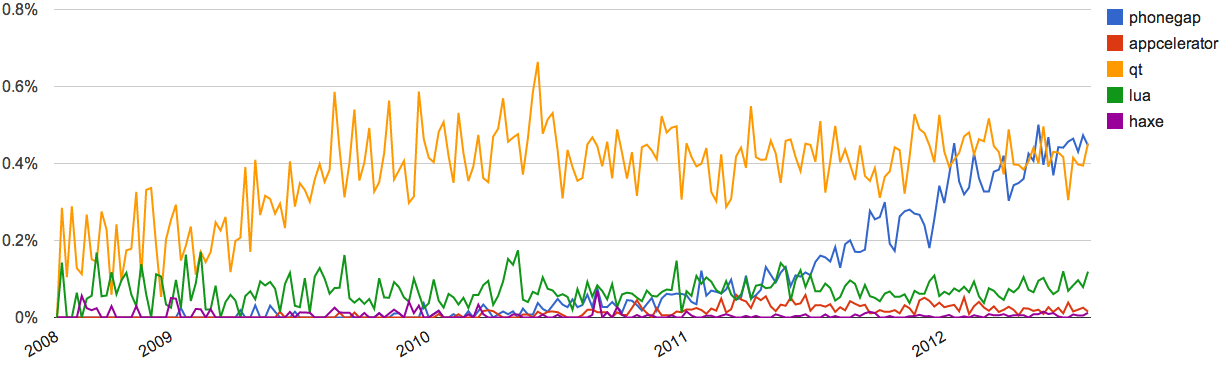
\includegraphics[width=\linewidth]{stackoverflow-trends}
 \caption{Prikaz trendov za nekaj od predlaganih rešitev na spletni strani Stackoverflow, kjer razvijalci iščejo rešitve problemov na katere so naleteli.}
 \label{fig:stackoverflow-trends}
\end{figure}

Vse omejitve omenjene v prejšnjem poglavju so predstavljene v tabeli \ref{table:omejitve}. Prazne vrstice pri ``grafični skladnosti'' za Lua, Haxe, C++ in JavaScript so posledica nezmožnosti zadoščanja te omejitve, niso pa ovira, saj mora v tem primeru za grafično skladnost poskrbeti domorodna koda, ki ni napisana v omenjenih jezikih.

Iz tabele \ref{table:omejitve} je lepo razvidno, da edino rešitev C++ zadošča vsem naštetim omejitvam. Poglejmo si torej kako lahko izbrano rešitev pripravimo s pomočjo jezika C++, ter kako lahko nato isto rešitev uporabimo tudi v aplikaciji, ki teče spletnem brskalniku, s pomočjo ogrodja Emscripten.

\begin{table}
\begin{tabular}{ l | c | c | c | c | c | c | c | c | c }
  \hline
  Omejitev/Rešitev & Qt & Xamarin & Air & Cordova & Titanium & Lua & Haxe & C++ & JavaScript \\
  \hline
  Android & \cmark & \cmark & \cmark & \cmark & \cmark & \cmark & \cmark & \cmark & \cmark \\
  iOS & \cmark & \cmark & \cmark & \cmark & \cmark & \cmark & \cmark & \cmark & \cmark \\
  Windows Phone & \xmark & \cmark & \xmark & \cmark & \xmark & \cmark & \cmark & \cmark & \cmark \\
  Spletna aplikacija & \xmark & \xmark & \cmark & \cmark & \xmark & \cmark & \cmark & \cmark & \cmark \\
  Grafična skladnost & \xmark & \cmark & \xmark & \xmark & \cmark &  &  & &  \\
  Skupnost & \cmark & \cmark & \xmark & \cmark & \cmark & \cmark & \xmark & \cmark & \cmark \\
  Odpornost na nadgradnje & \xmark & \xmark & \xmark & \xmark & \xmark & \xmark & \xmark & \cmark & \xmark \\
  Cena (mesečno) & 149\$ & 299\$ & - & - & - & - & - & - & - \\
  \hline
\end{tabular}
\label{table:omejitve}
\caption{Pregled funkcionalnosti posametnih rešitev.}
\end{table}

%-----
\section{C++}

Izbrani del RRULE specifikacije RFC 5545 je na srečo dovolj preprost, da za razvoj potrebujemo le STL (Standard Template Library) knjižnico. V kolikor bi naša rešitev zahtevala vključitev dodatne knjižnice, recimo vzpostavitev internetne povezave, bi lahko ta problem rešili na dva načina:

\begin{enumerate}
  \item V našo rešitev bi vključili dodatno knjižnico \texttt{libcurl}. To bi povzorčilo kar nekaj problemov pri vključevanju knjižnice na različne platforme, saj bi morali knjižnico \texttt{libcurl} pripraviti za vsak platformo posebej.
  \item Nalogo vzpostavitve in prenosa podatkov iz oddaljene lokacije bi lahko delegirali v domorodno kodo, ki bi po prenosu rezultat prenesla nazaj v našo knjižnico.
\end{enumerate}

Če izberemo prvi način, bo naša knjižnica podvajala funckionalnost, ki že obstaja v domorodni kodi. Veliko lepša rešitev je uporaba delegiranja v domorodno kodo, saj lahko ta boljše izkorišča vse sposobnosti naprave. To sicer pomeni nekaj več kode v ovojih naše knjižnice (kar si bomo ogledali v 4. poglavju), a omogoča boljšo odpornost na nadgradnje operacijskega sistema destinacijske platforme.

Razvito knjižnico lahko v platformske aplikacije vključimo na več različnih načinov:

\begin{enumerate}
  \item Z izvorno kodo C++, ki jo ciljni program vključi v svoj paket.
  \item Statično knjižnico (\eng{static library}), ki jo ciljni program vključi v svoj paket.
  \item Deljeno knjižnico (\eng{shared library}), ki jo ciljni program samo referencira, a jo ne vključi direktno v svoj paket.
\end{enumerate}

Pri vseh naštetih načinih je potrebna dodatna ovojna koda (\eng{wrapper}), ki je različna za vsako destinacijsko platformo. Detajle teh ovojev si bomo ogledali v poglavju \ref{chap:cross-platform}.

Primer uporabe knjižnjice RRULE RFC 5545 lahko vidimo v primeru \ref{code:cpp-primer}. Razred \texttt{Date} vsebuje vso potrebno logiko za delo z datumi, kot so naprimer prištevanje, odštevanje ter primerjanje datumov. Razred \texttt{Recurrence} vsebuje logiko za ponavljanje dogodkov. Tip dogodka, ki se ponavlja, je poljuben in ni del knjižnjice.

\begin{lstlisting}[caption={Primer uporabe C++ knjižnjice RRULE standarda RFC 5545. Izbrani dogodek bi se s tem pravilom ponavljal tedensko, vsak ponedeljek, od 1. januarja 2014 naprej.}, label=code:cpp-primer, language=C++]
Recurrence rec = Recurrence(Weekly, Date(2014, 1, 1));
rec.setByDay("MO");
map<int, Date> days = rec.daysInRange(Date(2014, 2, 1), Date(2014, 2, 28));
// spremenljivka days bo vsebovala
// result[5] = Date(2014, 2, 3);
// result[6] = Date(2014, 2, 10);
// result[7] = Date(2014, 2, 17);
// result[8] = Date(2014, 2, 24);
\end{lstlisting}

%==============================
\chapter{Vključitev knjižnice v različne platforme}
\label{chap:cross-platform}

%-----
\section{iOS}

Platforma iOS primarno uporablja jezik Objective-C, ki je, kot ime namiguje, objektna razširitev jezika C. Na srečo obstaja tudi variacija Objective-C++, ki nam omogoča souporabo jezikov Objective-C in C++ v istem projektu. Datoteki, v kateri želimo uporabljati C++, namesto končnice \texttt{.m} pripnemo končnico \texttt{.mm}.

iOS ne podpira uporabe deljene knjižnice (\eng{shared library}), omogoča pa uporabo statične knjižnice (\eng{static library}) ali izvorne kode. Za prvi primer izberimo uvoz izvorne kode.

iOS v svojem arsenalu ne vključuje orodje za avtomatično sproščanje pomnilnika (\eng{garbage collection}). Od razvijalca se pričakuje, da za seboj počisti pomnilnik z uravnoteženimi ukazi \texttt{retain} in \texttt{release}, ko je koda opravila svoje delo. V ta namen je v integriranem razvijalskem okolju (\eng{Integrated Development Environment}) XCode na voljo kar nekaj orodij, ki nam omogočajo lažjo detekcijo puščanja pomnilnika (\eng{memory leak}). Kar rado se zgodi, da se pri štetju referenc razvijalec zmoti. Na srečo je v iOS5 Apple predstavil ARC (avtomatično štetje referenc - \eng{Automatic Reference Counting}) s čimer so razvijalcem znatno olajšali delo, saj prevajalnik sedaj zna sam vnesti ukaze za sproščanje pomnilnika.

Implementacija iOS ovoja je dokaj preprosta (glej primer \ref{code:ios-wrapper}). Za vsakega C++ od razredov naredimo zrcalne Objective-C++ ovojne razrede, ki v inicializacijski metodi \texttt{init} poskrbijo za pravilno dodeljevanje in hranjenje C++ objekta (vrstica 14). Ko na določen objekt ne kaže več noben kazalec, se pred sprostitvijo pomnilnika pokliče metoda \texttt{dealloc}, v kateri poskribmo za ustrezno sprostitev C++ objekta predno pride do puščanja pomnilnika (vrstica 21). Klic v ovoj nato preprosto posreduje klic v C++ objekt (vrstica 25) in poskrbi za transformacije med C++ in Objective-C podatkovnimi tipi.

\lstset{language=[Objective]C, breaklines}
\begin{lstlisting}[caption={Primer Objective-C++ ovoja C++ razreda \texttt{Date}.}, label=code:ios-wrapper]
#import "ThesisDate.h"
#import "Date.hpp"

@interface ThesisDate() {
    Thesis::Date* wrapped;
}
@end

@implementation ThesisDate

- (ThesisDate *)initWithYear:(NSInteger)year month:(NSInteger)month andDay:(NSInteger)day {
    self = [super init];
    if (self) {
        wrapped = new Thesis::Date(year, month, day);
        if (!wrapped) self = nil;
    }
    return self;
}

- (void)dealloc {
    delete wrapped;
}

- (void)addDays:(NSInteger)days {
    wrapped->addDays(days);
}
\end{lstlisting}

%-----
\section{Android}

Java, ki jo srečamo na platformi Android, se od odprtokodne Jave kar precej razlikuje. Na površju za razvijalce morda ni opaziti razlike, a se veliko razlik skriva pod gladino. Android ne uporablja Java virtualnega pogona (\eng{Java Virtual Machine}) ampak svoj pogon Dalvik, ki je prilagojen za uporabo na mobilnih napravh. Pred kratkim je Google napovedal nov virtualen pogon, Android Runtime (ART), ki bo v prihodnosti zamenjal Dalvik in vsebuje veliko izboljšav v hitrosti in stabilnosti aplikacij.

Za izdelavo ovoja C++ kode moramo uporabiti dve orodji:

\begin{enumerate}
  \item JNI (Java Native Interface), ki poskrbi za komunikacijo med jezikoma Java in C++
  \item NDK (Native Development Kit), ki poskrbi za pravilno prevajanje C++ kode za vsako od ciljnih arhitektur Android platforme (armeabi, armeabi-v7a, x86 in mips).
\end{enumerate}

Uporaba orodja JNI je za razvijalca kar časovno potratna. Spisati je treba dva ovoja:

\begin{enumerate}
  \item Java ovoj, ki izpostavi C++ razrede in metode s pomočjo direktive \texttt{native} (glej primer \ref{code:android-java-wrapper}).
  \item C++ ovoj, ki služi kot most med jezikoma Java in C++, ter poskrbi za transformacije med podatkovnimi tipi (glej primer \ref{code:android-cpp-wrapper}).
\end{enumerate}

Referenco na C++ objekt hranimo v Java delu JNI ovoja, C++ ovoj pa do reference dostopa preko metode \texttt{getHandle} (glej \ref{code:android-cpp-wrapper}), ki spremenljivko \texttt{nativeHandle} poišče v Java delu JNI ovoja.

Java ovoje shranimo v direktorij \texttt{src}, medtem ko C++ JNI ovoje shranimo v \texttt{jni}. Poglejmo si kako poteka komunikacija med Javo in C++ v primeru klica \texttt{isBefore} (glej primer \ref{code:android-cpp-wrapper}):

\begin{enumerate}
  \item Java preko JNI najde pravo metodo v C++ ovoju s pomočjo dogovorjene poimenovalne sheme (vrstica 12)
  \item C++ ovoj pretvori Java argumente v C++ argumente (vrstica 14).
  \item C++ ovoj najde predhodno shranjen objekt (vrstice 40 - 44).
  \item Pokliče prailno metodo na najdenem objektu z C++ argumenti (vrstice 21 - 29).
  \item Če metoda vrne kak rezultat, C++ ovoj poskbi za pretvorbo nazaj v Java podatkovne tipe (vrstica 13).
\end{enumerate}

Bralca morda zanima čemu služi metoda \texttt{dispose} (vrstice 16-19). Java nam nudi avtomatično sproščanje pomnilnika (\eng{garbage collection}), medtem ko C++ od razvijalca zahteva samostojno čiščenje pomnilniških naslovov, ki niso več v uporabi. Ko v Javi pride do sproščanja pomnilnika, se pokliče metoda \texttt{finalize}, a kot lahko preberemo v dokumentaciji\cite{android-object} do klica ne prihaja prav pogosto in se za tako uporabo ne priporoča. Poleg tega je vsak razred, ki implementira metodo \texttt{finalize}, deležen malce večje obdelave iz strani operacijskega sistema, kar botruje počasnejšemu izvajanju. Ker želimo biti malce bolj prijazni do platforme na kateri gostujemo, se držimo pravila: ko objekta ne potrebuje več, ga sprostimo s pomočjo klica \texttt{dispose} (naprimer v \texttt{finally} \texttt{try catch finally} konstruktu).

\begin{lstlisting}[caption={Primer Java ovoja C++ razreda \texttt{Date}.}, label=code:android-java-wrapper, language=Java]
public class Date
{
	private long nativeHandle = 0;
	public native void init(int year, int month, int day);
	public native boolean isBefore(Date date);
	public native void dispose();

	public Date(int year, int month, int day) {
		init(year, month, day);
	}

	static {
		System.loadLibrary("thesis");
	}
}
\end{lstlisting}

\begin{lstlisting}[caption={Primer mosta med jezikoma Java in C++ razreda \texttt{Date}.}, label=code:android-cpp-wrapper, language=C++]
#include "info_hribar_thesis_Date.h"
#include "Date.cpp"

using namespace Thesis;

JNIEXPORT void JNICALL Java_info_hribar_thesis_Date_init(JNIEnv *env, jobject obj, jint year, jint month, jint day) {
	Date *date = new Date(year, month, day);
	setHandle(env, obj, date);
}

JNIEXPORT jboolean JNICALL Java_info_hribar_thesis_Date_isBefore(JNIEnv *env, jobject obj, jobject compare) {
	Date *date = getHandle<Date>(env, obj);
	return date->isBefore(getDate(env, compare));
}

JNIEXPORT void JNICALL Java_info_hribar_thesis_Date_dispose(JNIEnv *env, jobject obj) {
	Date *date = getHandle<Date>(env, obj);
	delete date;
}

Date getDate(JNIEnv *env, jobject date) {
	jclass dateCls = env->GetObjectClass(date);
	jmethodID mGetYear = env->GetMethodID(dateCls, "getYear", "()I");
	jmethodID mGetMonth = env->GetMethodID(dateCls, "getMonth", "()I");
	jmethodID mGetDay = env->GetMethodID(dateCls, "getDay", "()I");
	jint year = env->CallIntMethod(date, mGetYear);
	jint month = env->CallIntMethod(date, mGetMonth);
	jint day = env->CallIntMethod(date, mGetDay);
	return Date(year, month, day);
}

jfieldID getHandleField(JNIEnv *env, jobject obj)
{
    jclass c = env->GetObjectClass(obj);
    // J is the type signature for long:
    return env->GetFieldID(c, "nativeHandle", "J");
}

template <typename T>
T *getHandle(JNIEnv *env, jobject obj)
{
    jlong handle = env->GetLongField(obj, getHandleField(env, obj));
    return reinterpret_cast<T *>(handle);
}

template <typename T>
void setHandle(JNIEnv *env, jobject obj, T *t)
{
    jlong handle = reinterpret_cast<jlong>(t);
    env->SetLongField(obj, getHandleField(env, obj), handle);
}
\end{lstlisting}

%-----
\section{Windows Phone}

Primarni jezik vseh Windows platform je C\#, in isto velja tudi za Windows Phone. Z 8. verzijo mobilnega operacijskega sistema je Microsoft odprl možnost souporabe C++ in domorodne kode. To storimo z uporabo Windows Phone Runtime komponente (WinPRT), ki jo spišemo v jeziku C++, to pa nato uvozimo v naš Windows Phone projekt kot zunanjo referenco.

Našo knjižnico lahko uvozimo kot statično knjižnico (\eng{static library}), ali direktno kot C++ izvorno kodo (če imamo do nje dostop). Če se odločimo za uporabo statične knjižnice, moramo paziti, da ta uporablja le standardno knjižnjico (\texttt{STL}) in \texttt{Win32} klice, ki so dovoljeni za Windows Phone aplikacije\cite{windows-static}.

Funkcionalnost, ki jo rabimo v naši Windows Phone 8 aplikaciji, izvozimo v WinPRT C++ komponenti (glej primer \ref{code:wp8-wrapper}).

\lstset{language=[Sharp]C, breaklines}
\begin{lstlisting}[caption={C++ koda za izvoz funckionalnosti knjižnice v JavaScript razreda \texttt{Date}.}, label=code:wp8-wrapper, language=c++]
namespace ThesisWINRT {
    using namespace Windows::Foundation;
    using Platform::String;

    public ref class Date sealed {
    public:
        unsigned int GetLength(String^ strToParse);
    };
}
\end{lstlisting}

%-----
\section{Spletna aplikacija}

C++ knjižnico moramo za uporabo v spletni aplikaciji prevesti v JavaScript. To lahko storimo s pomočjo orodja emscripten, ki vzame LLVM zlogovno kodo in namesto prevoda v nabor ukazov za podprte procesorje, prevede to kodo v JavaScript. Rezultat je knjižnjica, ki jo lahko brez težav uvozimo v obstoječo spletno aplikacijo.

Primarno emscripten prevaja celotne programe, ki imajo jasno definirane vhode in izhode. Te lahko v JavaScriptu sprožimo kot bi jih v uporabniški vrstici (\eng{terminal}). V našem primeru gre vendarle za prevod C++ knjižnjice, za kar emscripten potrebuje dodatna navodila za izvoz funkcionalnosti (glej primer \ref{code:emscripten-bindings}). Za te namene projekt emscripten vsebuje \texttt{embind}\cite{emscripten-embind}, s pomočjo katerega lahko izvozimo dostop do razredov, podatkovnih tipov, pomnilniškim upravljanje in podobne jezikovne konstrukte.

\begin{lstlisting}[caption={C++ koda za izvoz funckionalnosti knjižnice v JavaScript razreda \texttt{Date}.}, label=code:emscripten-bindings, language=c++]
#include "emscripten/bind.h"
#include "src/Date.hpp"

using namespace emscripten;
using namespace Thesis;

EMSCRIPTEN_BINDINGS(date) {
    class_<Date>("Date")
        .constructor<int, int, int>()
        .property("year", &Date::getYear, &Date::setYear)
        .property("month", &Date::getMonth, &Date::setMonth)
        .property("day", &Date::getDay, &Date::setDay)
        .function("setDate", &Date::setDate)
        .function("addDays", &Date::addDays)
        .function("addMonths", &Date::addMonths)
        .function("addYears", &Date::addYears)
        .function("toString", &Date::toString)
        .function("isBefore", &Date::isBefore)
        .function("isAfter", &Date::isAfter)
        .function("isEqual", &Date::isEqual)
        .function("getWeekday", &Date::getWeekday)
        .function("isLastDay", &Date::isLastDay);
}
\end{lstlisting}

Končni rezultat izvoza knjižnice v JavaScript lahko vidimo v primeru \ref{code:javascript-date}.

\begin{lstlisting}[caption={Primer uporabe izvoženega razreda \texttt{Date} v JavaScript.}, label=code:javascript-date, language=JavaScript]
var date = new Thesis.Date(2014, 10, 10);
date.addMonths(1);
console.log(date.toString());
\end{lstlisting}